\chapter{Nuclear Stability and the Liquid Drop Model}

\section{Introduction}

In lecture 1 we saw that most nuclides are unstable and there is just a small ``island'' of stability in $N$ and $Z$ which is illustrated by the Segre Chart.  How can this be explained?

\section{Nuclear binding energy}

A nucleus has less mass than the sum of its individual nucleons. You can think of the binding energy of a nucleus as the energy {\em released} when the constituent protons and neutrons are brought together.  You can also think of the binding energy as the energy {\em required} to separate a nucleus into its constituent protons and neutrons. 

The difference in mass between the nucleus and its constituent protons and neutrons is called the {\em mass defect}. The higher the mass defect, the greater the energy release when constituent nucleons are brought together/the greater the energy required to separate nucleus into constituent nucleons.

Data sources (books, websites, exams!) usually provide atomic masses, but not always.  To obtain nuclear masses from atomic masses we need to subtract the masses of the electrons for a given atom.  We should also include the binding energy of the electrons, but this term is usually negligible compared to the binding energy of the nucleus:
\beq
M_{N} c^2 = M_A c^2 - Z m_e c^2 + \sum_i^Z B_i\,,
\eeq
where $M_N$ is the nuclear mass, $M_A$ the atomic mass, $m_e$ the mass of the electron and $B_i$ the binding energy of the $i^{th}$ electron.  Electronic binding energies are typically $10 -100$ keV whereas atomic mass energies are of order $A\times$1000 MeV, so it is usual to neglect the former.

The nuclear binding energy $B$ is then given by:
\beq \label{eqn:be0}
{B} = \left\{ Z m_p + N m_n - M_N (^A {\rm X}) \right\} c^2\,.
\eeq
or in terms of the atomic mass
\beq \label{eqn:be1}
{B} = \left\{ Z m_p + N m_n - \left[M_A (^A {\rm X})- Z m_e \right] \right\} c^2\,.
\eeq
Note that we can re-write this in the form:
\beq \label{eqn:be2}
{B} = \left\{ N m_n + Z M_A (^1 {\rm H})  - M_A (^A {\rm X})\right\} c^2\,,
\eeq
which can be slightly easier to handle when making calculations if you have atomic masses available.

\begin{careful}
Check what type of mass you are given in a question. Typically they will be atomic masses, but not always. 
\end{careful}

\begin{worked}{h!}{Energy Release Example}
Question: Derive an expression for the energy release, $Q$, in terms of the binding energy of the parent nucleus, $X$, and daughter nucleus, $Y$, when $X$ decays via $\beta^{-}$ emission.

\solution{Solution: See end of chapter.}
\end{worked}

We will now perform two examples of writing the energy release, $Q$, in terms of the binding energies.

\begin{worked}{h!}{Energy Release Example}
Question: Repeat the previous example when $X$ decays via $\beta^{+}$ emission.

\solution{Solution: See end of chapter.}
\end{worked}

\subsection{Binding energy per nucleon}

 From Eqns.~(\ref{eqn:be1}) and~(\ref{eqn:be2})   we can easily calculate the binding energy per nucleon ($B/A$) and plot this against mass number $A$, as shown in Fig.~\ref{fig:binding}.

\begin{example}{Binding Energy Per Nucleon Example}
The mass of a neutron and proton are 1.00866 u and 1.00728 u respectively, where 1 atomic mass unit (u) is ${\rm 931.5 {\rm MeV/c}^2}.$ The {\em nuclear} mass of an alpha particle is 4.00153 u. The mass defect is then 2*1.00866 u + 2*1.00728 u - 4.00153 u = 0.03035 u = 28.3 ${\rm MeV/c^2}$. Converting this to energy by multiplying by $c^2$, the binding energy is 28.3 MeV, or 7.1 MeV per nucleon.
\end{example}

\begin{figure}[h]
\centering
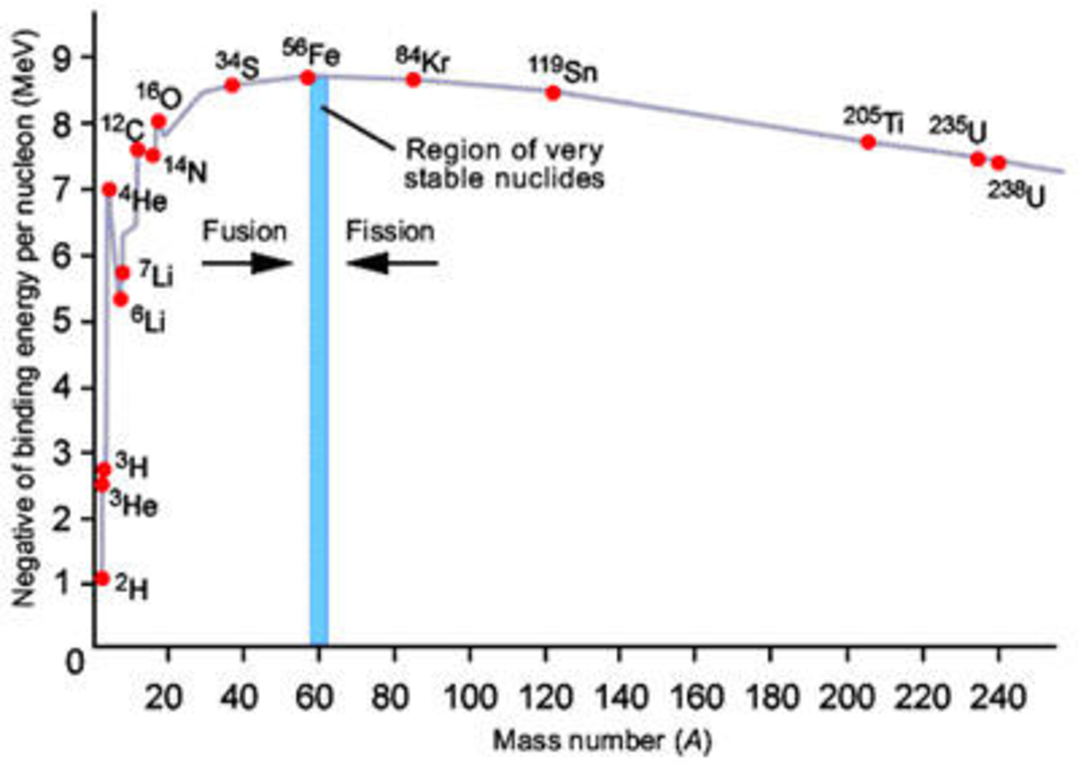
\includegraphics[width=0.8\columnwidth]{plots/bindingenergy.pdf}
\caption{\label{fig:binding} The binding energy per nucleon ($B/A$) versus mass number $A$ for stable nuclei.}  
\end{figure}

We note that the curve reaches a maximum near $A = 60$, where the nucleons are most tightly bound.  This suggests that we can release this binding energy in one of two ways.  For $A<60$ we can assemble lighter nuclei into heavier nuclei and for $A>60$ we can break heavier nuclei into lighter nuclei.  These processes are known, respectively, as nuclear fusion and nuclear fission.  We will discuss them in greater detail later.  The other remarkable feature is that for $A>16$ the binding energy per nucleon is within 10\% of 8 MeV.
